\documentclass{beamer}

%\usepackage{default}
%\usetheme{Berkeley}
\usetheme{Ilmenau}
\usecolortheme{beaver}
\usepackage[utf8]{inputenc}
\usepackage{caption}
\usepackage{pslatex}
\usepackage{textpos}
\usepackage{tikz}
%\useoutertheme{split}
%\useoutertheme{sidebar}
\usepackage{graphicx}
\pgfdeclareimage[height=2.35ex,width=2.2\baselineskip]{barcmini}{./PICS/barc_logo_circle.png}
\logo{\pgfuseimage{barcmini}}
\setbeamertemplate{sidebar right}{} %
\setbeamertemplate{footline}{\raisebox{-1ex}{\pgfuseimage{barcmini}}
    \usebeamerfont{date in head/foot} \@CERN \;\;\;\; \insertshortdate{}\hfill 
    \usebeamerfont{author in head/foot}\insertshortauthor{}\hfill
    \usebeamertemplate{navigation symbols}\hfill 
    \insertframenumber{}/\inserttotalframenumber
}
%\setbeamertemplate{navigation symbols}{}
\title{TARC Analysis using Geant4}
\author{Abhijit Bhattacharyya}
\institute{Bhabha Atomic Research Center \\ Mumbai INDIA}
\date{Aug 21, 2018}
%\logo{
\includegraphics[height=1cm,width=1cm]{../PICS/barc_logo_circle.png}}

\begin{document}
    \begin{frame}
        \maketitle
    \end{frame}

    \begin{frame}
        \frametitle{Outline}
        \begin{itemize}
            \item Why TARC ?
            \item TARC Basics.
            \item The Role of BARC. 
            \item Geant4 Results.
        \end{itemize}        
    \end{frame}

    \begin{frame}
    \frametitle{Why TARC?}
    First experiment $<$ PS-211 $>$ (TARC) was conceptualized by Carlo Rubbia and his collaborators at CERN-PS.
    \pause
        \begin{itemize}
            \item<1-> Nuclear waste management transforming transuranic isotopes.
            \pause
            \item<2-> Production of new radio-isotopes by neutron capture for medical importance [\textit{e.g.} for cancer treatment] using accelerator driven system (ADS).
            \pause
            \item<3-> Transformation of actinides by fission and thereby producing energy [\textsl{Energy Amplifier}] using a fast neutron sub-critical system driven by proton accelerator.
        \end{itemize}
    \end{frame}

    \begin{frame}
        \frametitle{Initial ideas}
        The discovery of the Spallation technique by Goeckerman and Perlman ({\tiny \textit {ref: Phys. Rev 73, 1127 (1948)}}) influenced Lewis ({\tiny \textit{ref: Report AECL-968 (1952)}}) to suggest the use of high current proton accelerators for the purpose of breeding fissile $^{233}$U or $^{239}$Pu from the fertile $^{232}$Th or $^{238}$U respectively.
         \begin{figure}
            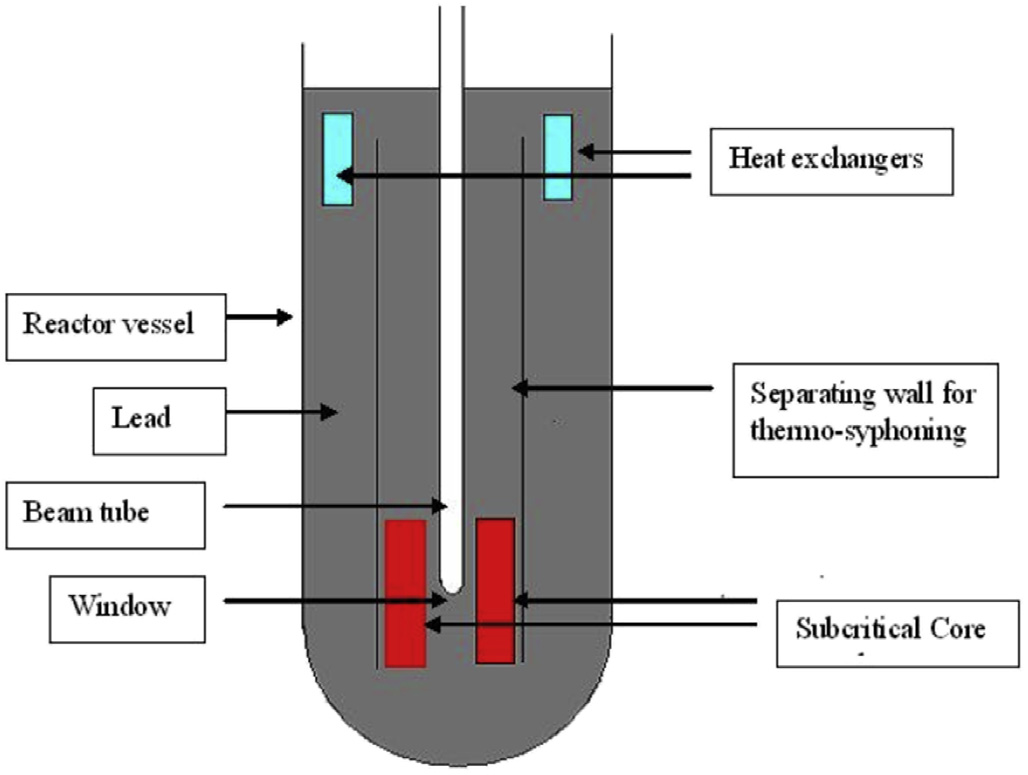
\includegraphics[height=40mm, width=80mm] {PICS/CERN_initial_concept.png} \label{fig:cern_tarc_reactor_concept_1995}
            \caption{{\tiny {The first design proposal of the 600 MWe fast energy amplifier (EA) ADS of CERN for power production using Thorium fuel ({\tiny \textit{Ref: CERN/AT/95-55(ET)(1995)).}}}}}
        \end{figure}
    \end{frame}

    \begin{frame}
    \frametitle{TARC basics : Key components}
    \begin{itemize}
        \item <1> A proton accelerator which may be part of \textit{ADS} (accelerator driven system), 
        \pause
        \item <2> A heavy metal spallation target that may produce neutron when bombarded by high energy proton from accelerator.
        \pause
        \item <1-3> A sub-critical core containing fuel (solid or liquid) that is neutronically coupled to the spallation target. Higher fission cross section reduce principal isotopes like $^{239}$Pu.
    \end{itemize}
    \end{frame}

    \begin{frame}
    \frametitle{TARC basics : Key components}
    \small{
        Number of fission neutrons produced by multiplication of a single neutron injected in core = $\frac{\kappa}{1-\kappa}$.
        \vskip 3mm
        Let 1 fission produce $\nu$ fission neutrons.\\
        Source producing $S_0$ neutrons/second would produce $\frac{S_0 \kappa}{\nu \left(1-\kappa \right)}$ fission / sec.
        \vskip 3mm
        Let $e_f$ is power released / fission.\\
        Hence total power released = $\frac{e_f S_0 \kappa}{\nu \left(1-\kappa\right)}$ /second.
        \vskip 3mm
        For $\kappa_{eff}=0.95$ and $\kappa_{eff}=0.98$ the source strength must be of the order of $6.2 \times 10^{18}$ n/sec and $2.4 \times 10^{18}$ n/sec respectively to produce about 1500 MWt power i.e. the power of \textbf{Energy Amplifier}.
    }
    \end{frame}
       
    \begin{frame}
    \frametitle{TARC basics : Properties of spallation target}
    "Natural Lead" [1.4\% $^{204}$Pb, 24.1\% $^{206}$Pb, 22.1\% $^{207}$Pb, 42.4\%$^{208}$Pb] :  spallation target.
    \begin{itemize}

        \item <1> MeV region to thermal energy: Transparent to neutron.  
        
        {\small  Very low absorption cross section [$^{204}$Pb : 0.65b, $^{206}$Pb : 0.03b, $^{207}$Pb : 0.699b, $^{208}$Pb : 0.00046b].} 
        
        Lead also possess high and energy independent elastic scattering cross section (mean free path $\lambda$ $\sim$ 3cm) which means lead behaves as transparent to neutron.
        
        \item <2> {\small Moderate slowing down effect due to very small lethargic ($\xi$ $\approx$ $9.6 \times 10^{-3}$) steps of neutron.} 
        
        \item<3> {\small Below the capture resonance energy ($E_n$ $<$ 1 keV) down to epithermal energy, the elastic scattering process is nearly isotropic : ``long storage time" (3 ms time for about 1800 scatterings to cover a total path of about 60 m to thermalize 1 MeV neutron).}     
    
    \end{itemize}
    \end{frame}

    \begin{frame}
    \frametitle{TARC basics: Properties of spallation target}   
     
    \begin{figure}
        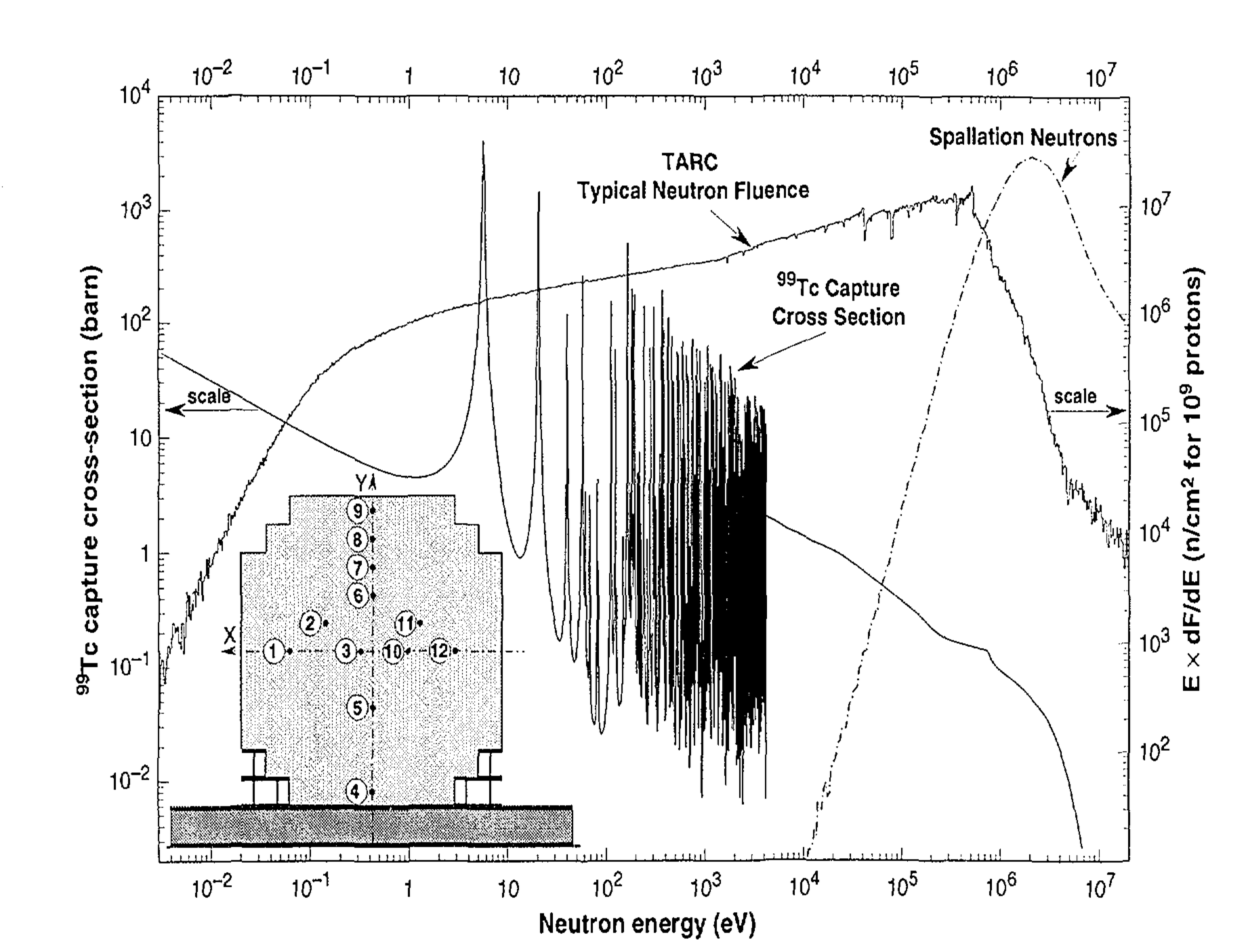
\includegraphics[height=45mm, width=80mm]{PICS/ED_Spallation.png} \label{fig:spallationtarget_1}
        \caption{{\tiny $^{99}$Tc capture cross section 4000b @ 5.6eV (vide JENDL 3.2 database) as a function of neutron energy (left hand scale), typical neutron fluence energy distribution in TARC (hole 10, z=+75 mm) as a function of neutron energy in isolethargic bins, for 3.5 $GeV/c$ protons (right hand scale), Energy distribution of neutrons from the spallation process.
        {\tiny \textit Ref: CERN 99-11 Dec 15, 1999: The TARC Experiment (PS-211) report }}}
    \end{figure}
    \end{frame}

    \begin{frame}
    \frametitle{TARC Experiment :: CERN}
    \begin{columns}
        \column[t]{55mm}
        \begin{itemize}
            \item Proton Beam : 2.5 GeV/c, 3.5 GeV/c
            \item 334 tons of Pb with dimension $3.3m \times 3.3m \times 3m$ block.
            \item Beam enters through a $77.2$ mm diameter, 1.2m long blind hole.
            \item $12$ sample holes are located inside the lead volume to measure capture cross sections of some samples. 
        \end{itemize}
        \column[t]{50mm}
        \begin{figure}
            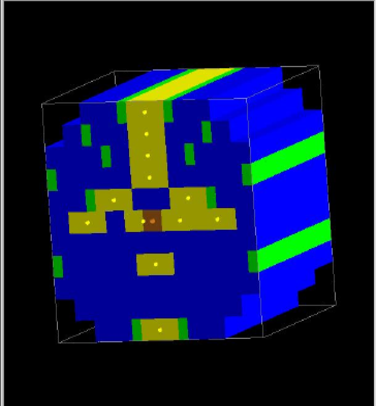
\includegraphics[height=50mm, width=45mm] {PICS/TARC_CERN_Lead.png}
        \end{figure}
    \end{columns}    
    \end{frame}

    \begin{frame}
    \begin{figure}
        \vskip -3mm
        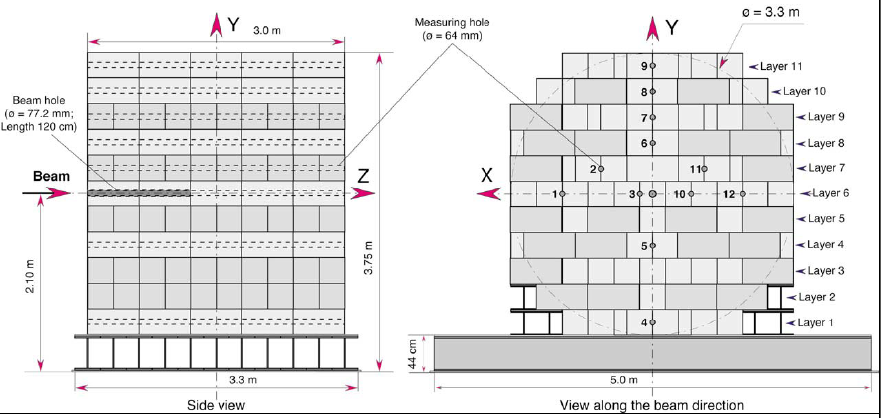
\includegraphics[height=70mm, width=115mm] {PICS/TARC_CERN_Lead_Assembly}
        \caption {TARC Lead Assembly {\tiny \textit Ref: CERN-SL-2001-033 EET, PS-211 REPORT}} 
    \end{figure}
    \end{frame}

    \begin{frame}
    \frametitle{The Role of BARC}
    The development at BARC has been conceptualized in three phases:
    \begin{itemize}
        \item A 20 MeV, 10 mA normal conducting front-end, called
        the Low Energy High Intensity Proton Accelerator.  
        \item A 200 MeV, 10 mA, superconducting accelerator using
        single-spoke resonators, called the Medium Energy High Intensity
        Proton Accelerator. 
        \item The full 1 GeV, 10 mA, CW, High Energy High Intensity
        Proton Accelerator, using elliptic cavities from 200 MeV to 1 GeV. 
    \end{itemize}
    \end{frame}

    \begin{frame}
    \frametitle{Geant4 Results : Validation}
    \begin{itemize}
        \item Spallation neutron production in lead target by protons,
        \item Validation of energy - time relationship for thermalization of neutrons,
        \item absolute neutron fluence variation over energy and radial distances verifying neutron transport properties.
    \end{itemize}
    \end{frame}

    \begin{frame}
    \frametitle{Geant4 Results : Distribution of Neutron Energy Deposition}
    \vskip -2mm
    \begin{figure}
    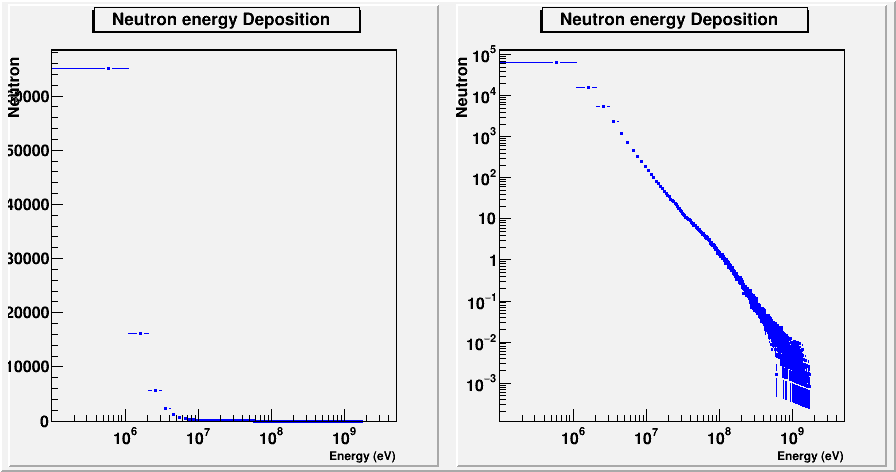
\includegraphics [height=30mm, width=85 mm] {PICS/NeutEdepBIC.png}
    \caption{\small QGSP\_BIC\_HP}
    \end{figure}
    \vskip -7mm
    \begin{figure}
    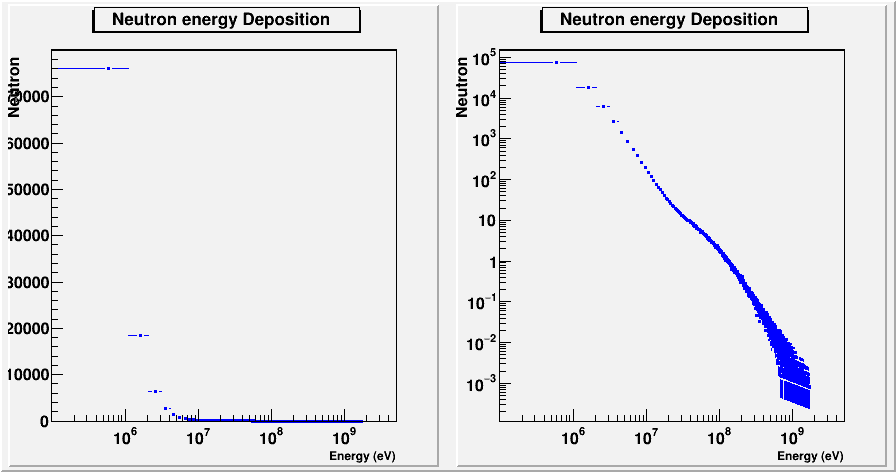
\includegraphics [height=30mm, width=85mm] {PICS/NeutEdepBERT.png}
    \caption{\small QGSP\_BERT\_HP}
    \end{figure}
    \end{frame}

    \begin{frame}
    \frametitle{Geant4 Results : Correlation of Neutron Energy - Time}
    %\begin{columns}[c]
        %\column[c]{0.5\textwidth}
    \vskip -2mm
    \begin{figure}
    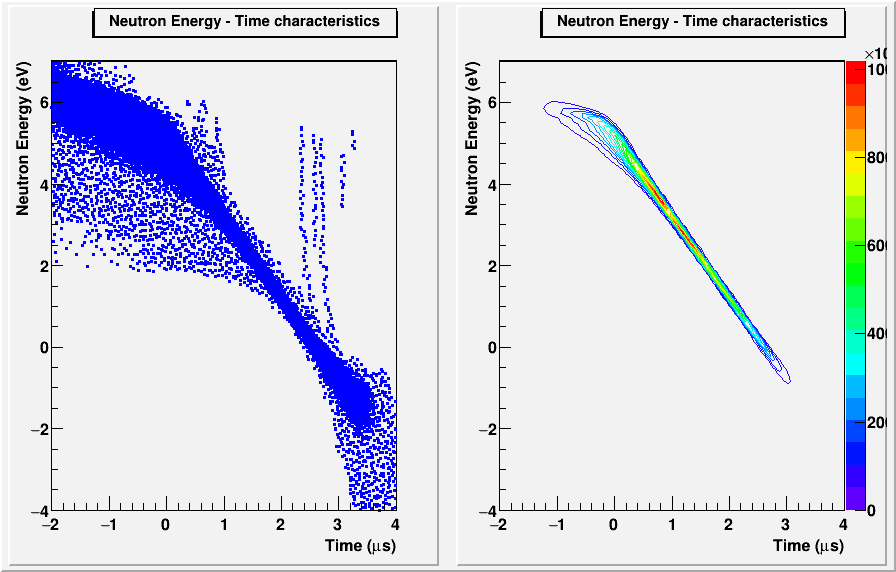
\includegraphics [height=30mm, width=85 mm] {PICS/NeutEnergyTimeBIC.png}
    \caption{\tiny QGSP\_BIC\_HP}
    \end{figure}
    \vskip -7mm
        %\column[c]{0.5\textwidth}
    \begin{figure}
    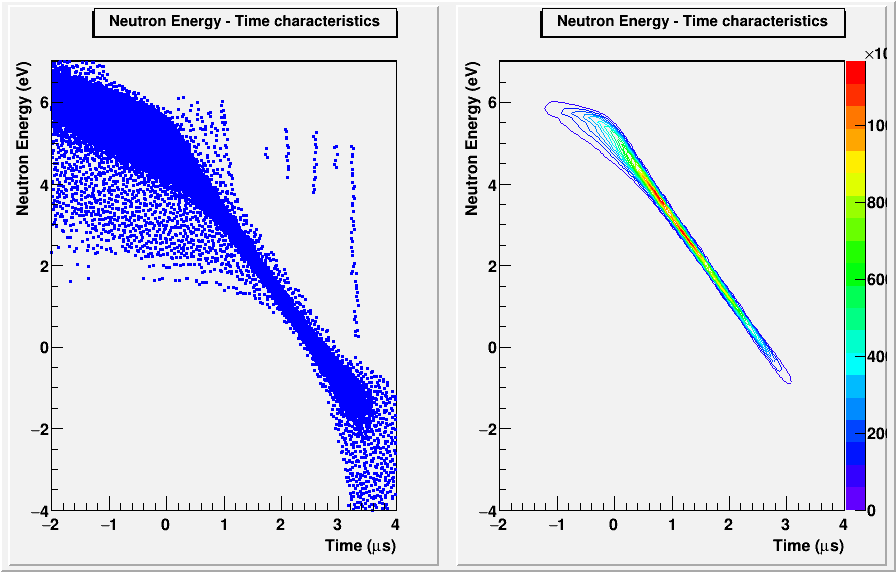
\includegraphics [height=30mm, width=85mm] {PICS/NeutEnergyTimeBERT.png}
    \caption{\tiny QGSP\_BERT\_HP}
    \end{figure}
    %\end{columns}
    \end{frame}

    \begin{frame}
    \frametitle{Geant4 Results :Correlation of Other particle Energy - Time}
    \vskip -2mm
    \begin{figure}
    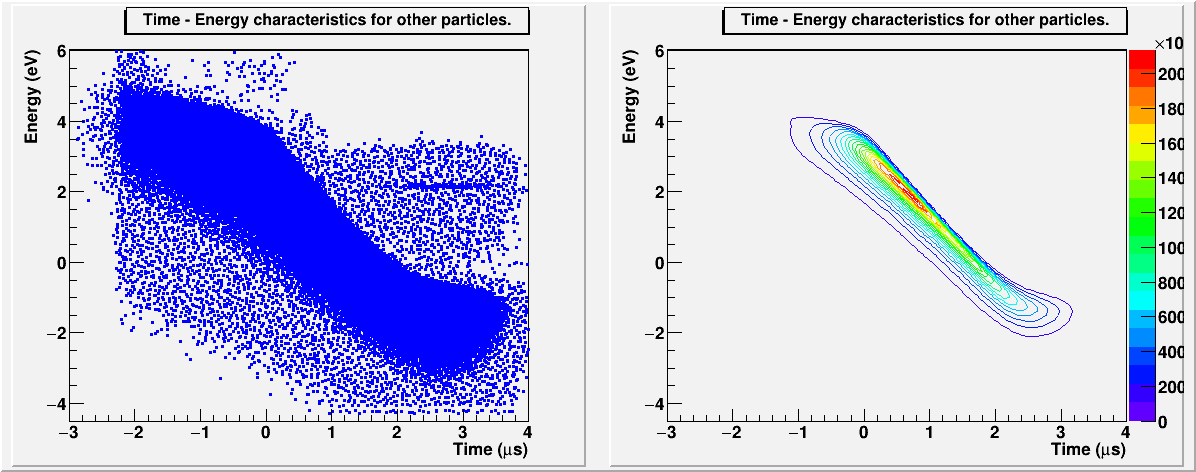
\includegraphics [height=30mm, width=85 mm] {PICS/OtherEnergyTimeBIC.png}
    \caption{\tiny QGSP\_BIC\_HP}
    \end{figure}
    \vskip -7mm        
    \begin{figure}
    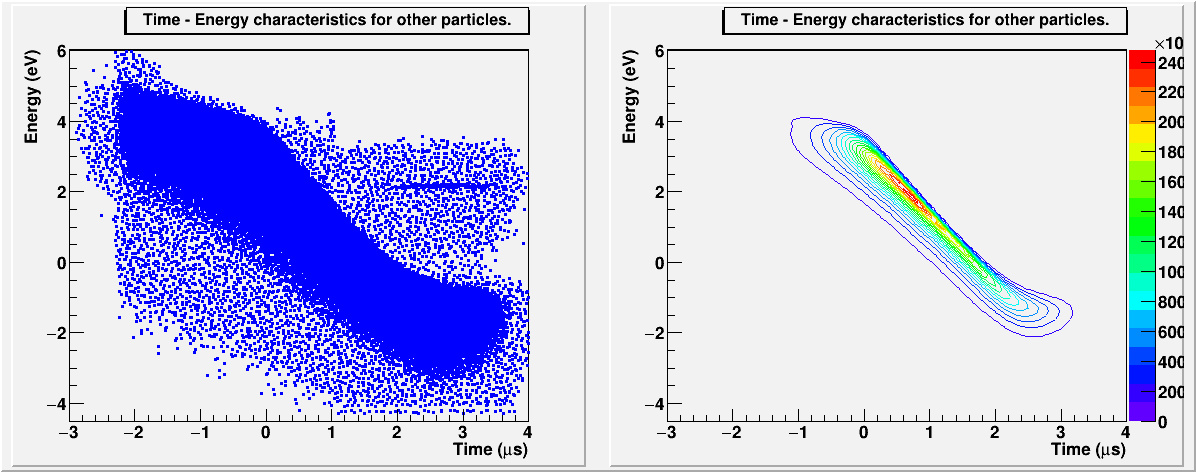
\includegraphics [height=30mm, width=85mm] {PICS/OtherEnergyTimeBERT.png}
    \caption{\tiny QGSP\_BERT\_HP}
    \end{figure}
    \end{frame}

    \begin{frame}
    \frametitle{Geant4 Results : Distribution of Fluence with Energy}
    \vskip -2mm
      \begin{columns}[c]
      \column[c]{0.5\textwidth }
        \begin{figure}
        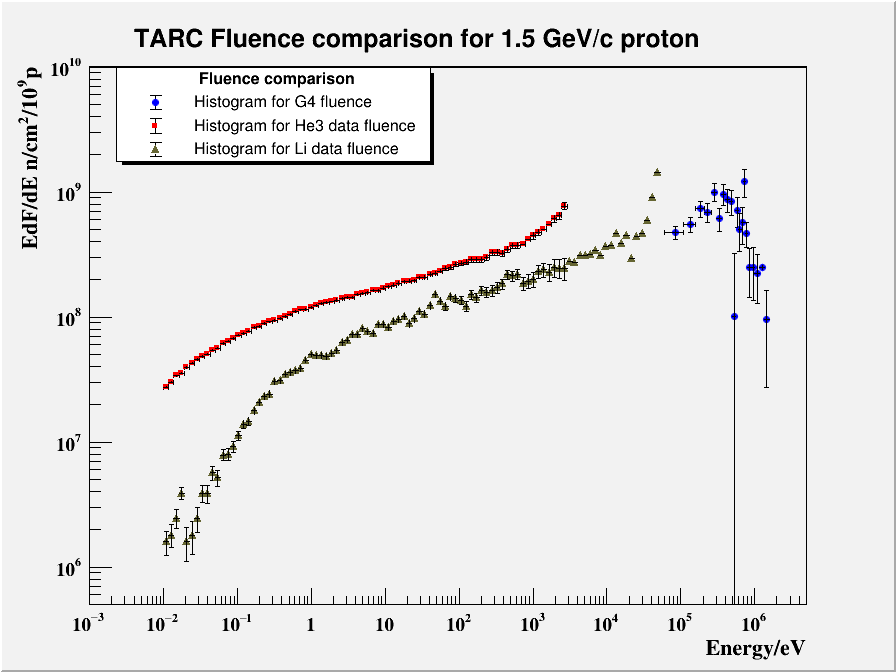
\includegraphics [height=30mm, width=60 mm] {PICS/FluenceEnergyBIC.png}
        \caption{\tiny QGSP\_BIC\_HP}
        \end{figure}

      \column[c]{0.5\textwidth }
        \begin{figure}
        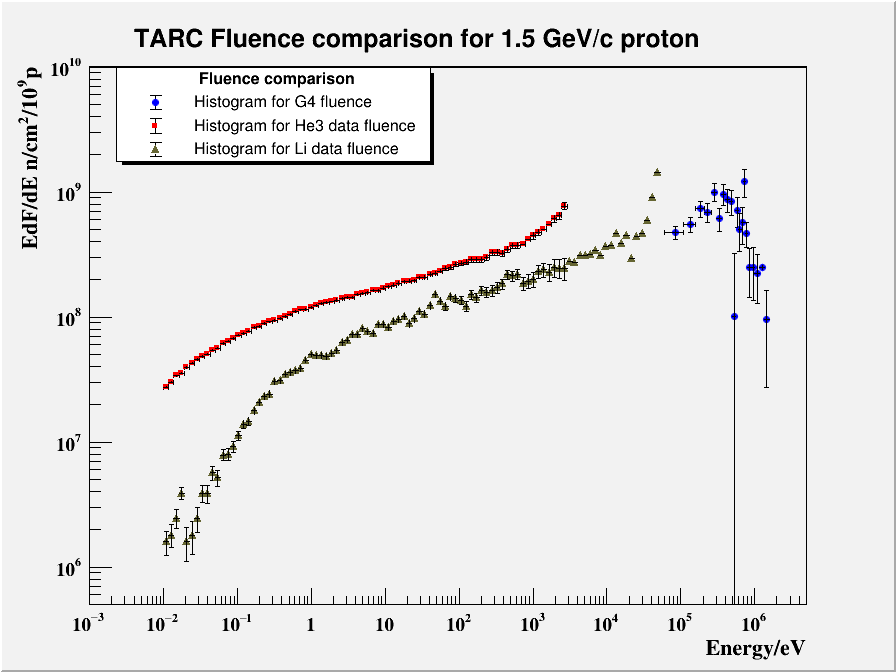
\includegraphics [height=30mm, width=60 mm] {PICS/FluenceEnergyBERT.png}
        \caption{\tiny QGSP\_BERT\_HP}
        \end{figure}
    \end{columns}
    \end{frame}

    \begin{frame}
    \frametitle{Geant4 Results : Distribution of Fluence with Radial distance from center}
    \vskip -2mm
    \begin{figure}
    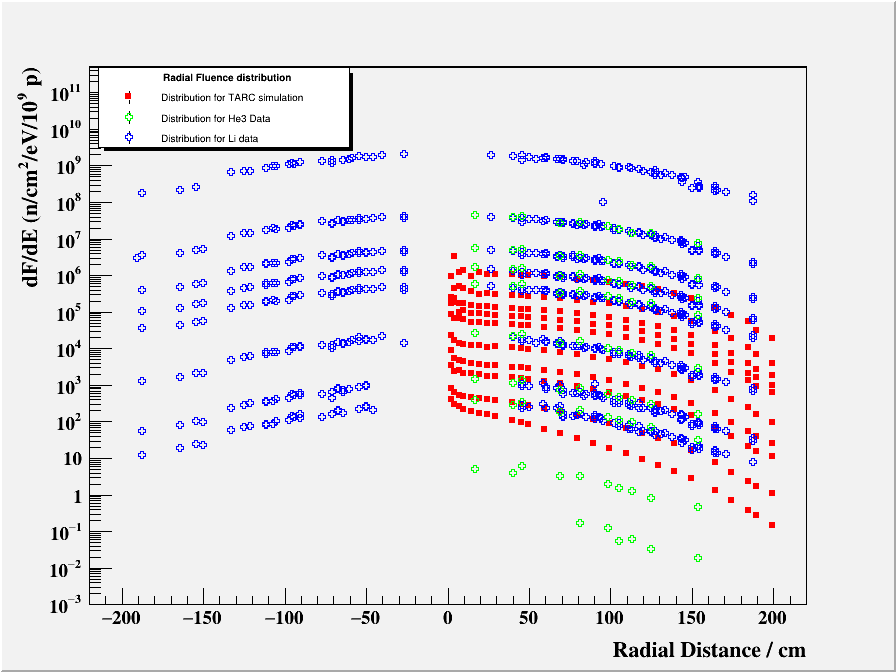
\includegraphics [height=30mm, width=85 mm] {PICS/FluenceRadialDistBIC.png}
    \vskip -2mm
    \caption{\tiny QGSP\_BIC\_HP}
    \end{figure}
    \vskip -7mm
    \begin{figure}
    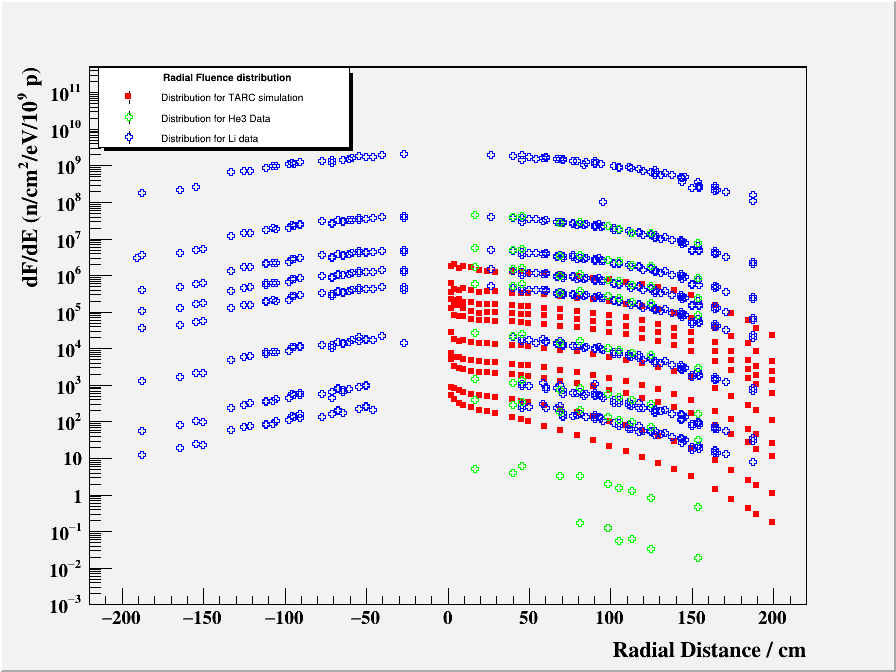
\includegraphics [height=30mm, width=85mm] {PICS/FluenceRadialDistBERT.png}
    \caption{\tiny QGSP\_BERT\_HP}
    \end{figure}
    \end{frame}

    \begin{frame}
    \frametitle{Geant4 Results : Ratio plot of Fluence G4/data}
    \vskip -3mm
    \begin{figure}
        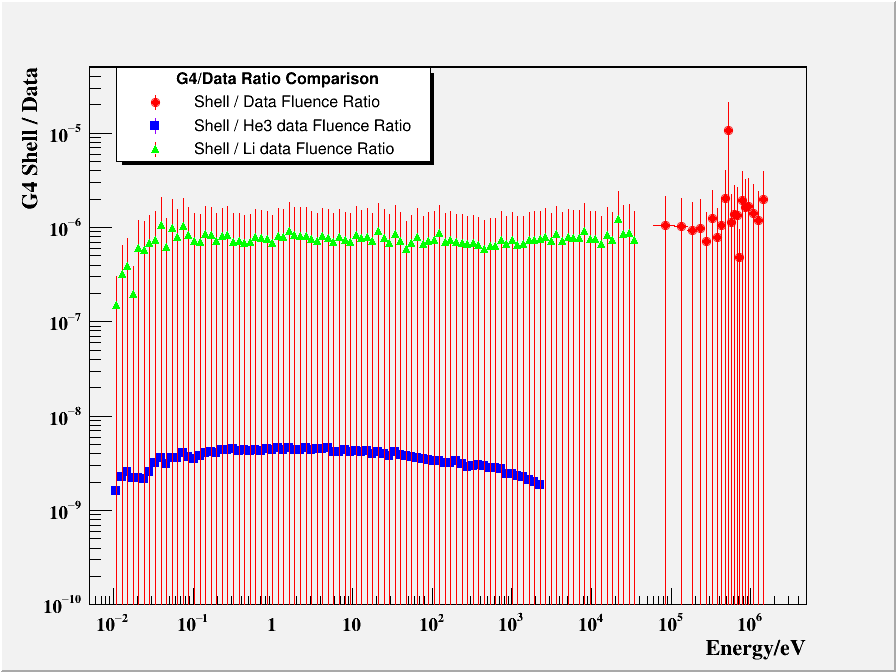
\includegraphics[height=30mm, width=80mm] {PICS/RatioBIC.png}
        \caption{\tiny QGSP\_BIC\_HP : Ratio of fluences for $4\pi$ shell:data}
    \end{figure}
    \vskip -7mm
    \begin{figure}
        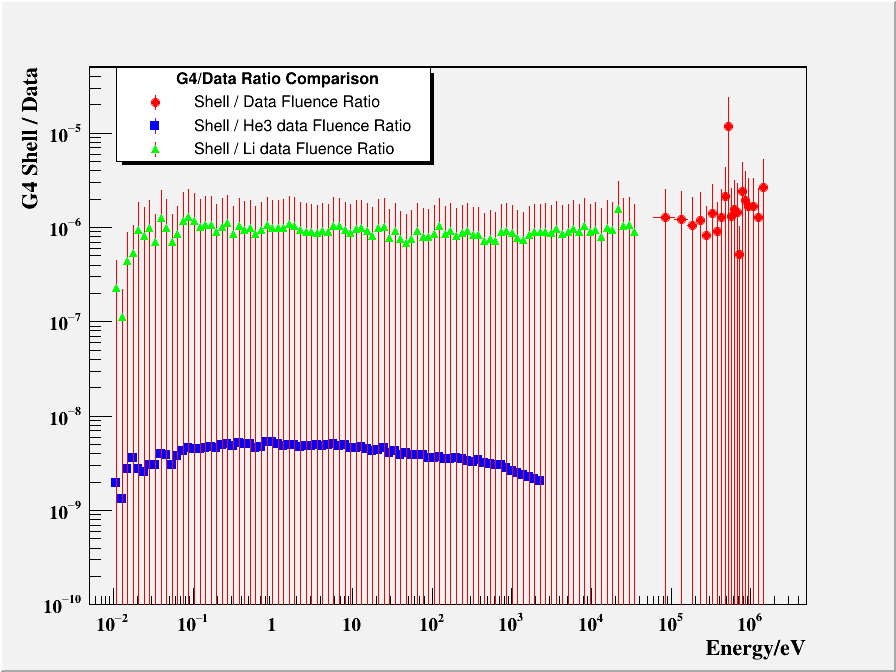
\includegraphics[height=30mm, width=80mm] {PICS/RatioBERT.png}
        \caption{\tiny QGSP\_BERT\_HP : Ratio of fluences for $4\pi$ shell:data}
    \end{figure}
    \end{frame}

    \begin{frame}
    \frametitle{Geant4 Results : Distribution of Flux}
    \vskip -2mm
    \begin{figure}
    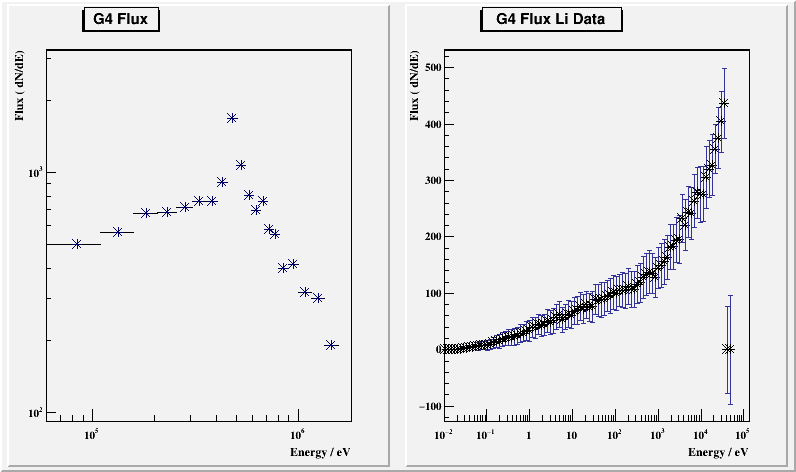
\includegraphics [height=30mm, width=95 mm] {PICS/FluxBIC.png}
    \vskip -2mm
    \caption{\tiny QGSP\_BIC\_HP}
    \end{figure}
    \vskip -7mm
    \begin{figure}
    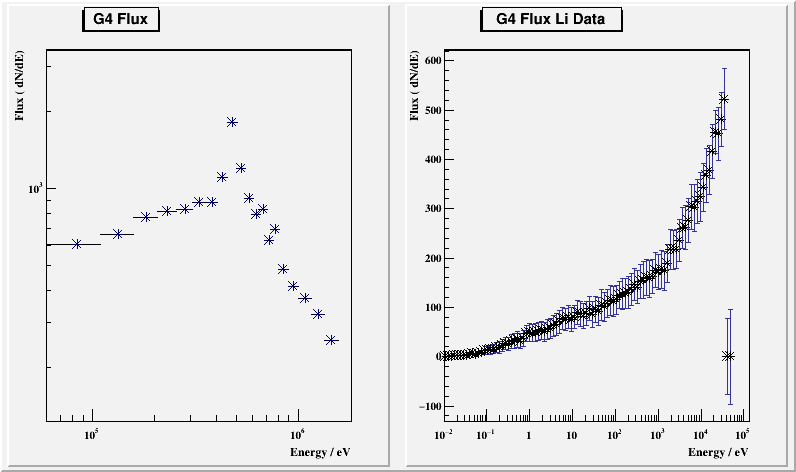
\includegraphics [height=30mm, width=95mm] {PICS/FluxBERT.png}
    \caption{\tiny QGSP\_BERT\_HP}
    \end{figure}
    \end{frame}

    \begin{frame}
    The following topics are either performed or in progress:\\
    (a) Studies like specific energy release per proton per $10^{10}$ protons at different positions.    \\
    (b) Breeding with $^{99}$Tc and $k\_{eff}$ calculations with neutron spectra and concentration of relevant element as a function of burn-up.
    
    \vskip 1cm
    
    \begin{center}
             \LARGE \textsl {Thank You}
    \end{center}
    \end{frame}

\end{document}